\section{投影和表示}

\subsection{太阳比喻}

在晴朗的日子里出去走一走,我们看不见自己,但却能看见自己的影子。这是很有意思的事情。

如果太阳不是很晒的话,我们可以站在一个空旷平坦的地上观察我们的影子,它和阳光射来的方向相对,在地上留下一个阴影,如果时间早的话,太阳升的不是很“高”,光线会斜斜地在地上投下一个较长的阴影,随着时间的流逝,太阳会沿着自己的轨道在天空中划出一个圆弧,随着太阳的升“高”,阴影会越来越短,当太阳升到最“高”的时候,阴影也最短。

但说高并不精确,我们可以把眼睛眯起,朝太阳的方向看,所谓“高”就是我们要仰起脖子才能“追踪”到太阳,我们仰起脖子的角度越大、太阳越高,我们可以把这个仰角定义为“太阳-观察者”连接线与地面的夹角$\theta$。当这个角度为$90^o$的时候,太阳在天顶,光线垂直地射下来,此时我们在地上的影子会“消失”\footnote{阴影之内没有光线是暗的,而阴影之外会被阳光照亮,光在这里更多地体现出“粒子性”,它以直线传播,绝对不会绕过障碍物。光从$\theta$方向照射到物体上,在地面上留下一个影子,假设物体的高度是$H$,影子的长度将是$H \cdot \frac{\cos \theta}{\sin \theta } = H \cdot \cot \theta$。}。

\begin{figure}[htbp]
\begin{center}
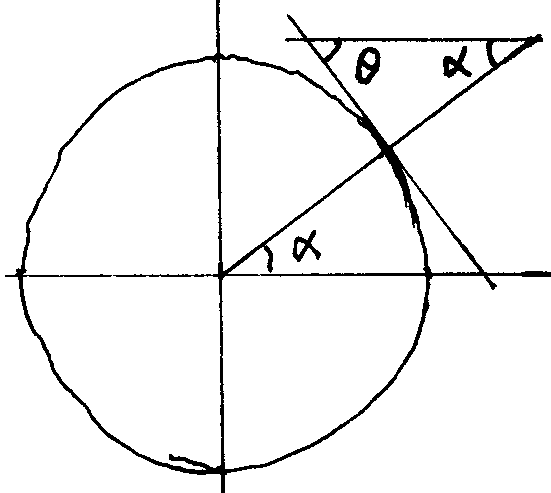
\includegraphics[width=5cm]{DiracNotation/sun_projection_1.png}
\caption{太阳光入射,与竖直方向成$\alpha$角。}
%\label{default}
\end{center}
\end{figure}


有时我们也以竖直的方向为基准,定义太阳光与竖直方向的夹角为$\alpha$($\alpha = \frac{\pi}{2} - \theta $),当$\alpha = 0$时,阳光笔直地照射在地面上,这时照射到单位面积上太阳光的能量最大,当角度$\alpha$逐渐增大时,照射到单位面积上太阳光的能量会变小,变小的比例正比于$\cos \alpha$。

人类走出非洲后,一路向北,先来到中近东,然后扩散到欧洲、亚洲等其它地方。中近东、欧洲、亚洲比非洲的纬度高,太阳会以一个更大的角度$\alpha$照射下来,随着$\alpha$的增大,单位表面积上地球吸收到的能量会减少,气温会随之降低,尤其是夜晚温度会更低。

我们现在都是住在屋子里的,但在远古人类甚至连制造房屋的技术都没有发明,冷了只能去山洞。但山洞里已经有其他动物占领了,比如曾广泛分布于欧洲和中近东各地的洞熊(cave bear)。洞熊的体型庞大,雄性洞熊的体重可高达1吨,可以想象与洞熊争夺山洞的战役是人类走出非洲后碰到的一大挑战。在这个过程中,火的使用是决定性的,因为在各种动物中只有人类不怕火,甚至还学会了使用火,发明了保存火种的方法,甚至制造火种的技术\footnote{维特鲁威在《建筑十书》中说:“远古时候,人类生来就像出没森林、洞穴和丛林中的野兽一样,茹毛饮血,辛苦度日。那时有一个地方,生长着密集繁茂的森林,狂风袭来,树木剧烈摇晃,树枝相互摩擦而起火。住在附近的人们被火焰吓坏了,逃之夭夭。但后来他们凑近时发现,火的热量对人体有极大的好处,他们将原木投入火中,将火种保存下来。”}。

可以想象人类曾长期生活在生有篝火的洞穴里,而这样的一个原始记忆也被用于比喻说理中,比如柏拉图在《理想国》中借用“洞穴”比喻了城邦和知识。

那么我们的洞穴经验是什么样的呢?

首先需要一个封闭的空间,比如在伸手不见五指的夜晚,任何一个房屋都可以是个洞穴,山洞无非也是个封闭的空间。

漆黑的夜晚,我们呆在山洞或封闭的房子里。我们什么都看不见,我们看不见自己,也看不见他人和物体。我们点燃一个火把或蜡烛。人是喜欢光亮的,于是都凑过去,此时我们在墙壁上看到影子,因为火把的光比较弱,反射一次后就基本没亮光了,洞穴中的影子会比阳光下的更显著和夸张,光和影在一起给我们的视觉极大的刺激。

阳光下我们不能清晰地看到物体的轮廓,但在洞穴经验中,阴影和光亮是截然分开的,我们甚至可以想象一个人去描摹阴影的轮廓。

用简单的线条去对象化一个物体是认识活动的开始,比如自我是不可见的,俗话说我们是在别人的眼睛(其实就是镜子)里认识自己的,但在洞穴经验里,我们在墙壁上能直接看见自己的阴影,比如我们可以面对着墙壁,背对着火把,伸出一只手,举过头顶……然后,我看见我面对的那个阴影会同步地作出这种种动作。

这就从视觉经验上把自我对象化了,同时我还能看见别人的阴影和其他物体的阴影……

火把的好处是可以随意移动,要想看清楚什么东西我们只需要把火把拿过来照一照就可以了。这意味着我们可以控制光线行进的方向,我可以让光向上方射,只需要我们把火把放在物体的下方,我们也可以让光向左射,只需要把火把放在物体的右边……

在洞穴中,我们举着火把从各个方向照物体,为的是要看清某物,光从某个方向射过来,我们看到的是光照亮的那个“面”,物体其他面的形象对我们是隐藏的,我们必须移动火把,使光从另外的方向射向物体,这个动作其实就是选择,我们选择从另一个角度“照亮”物体,刚才对我们显现的将隐藏在黑暗里,但新的面,新的形象会对我们显现。

\begin{figure}[htbp]
\begin{center}
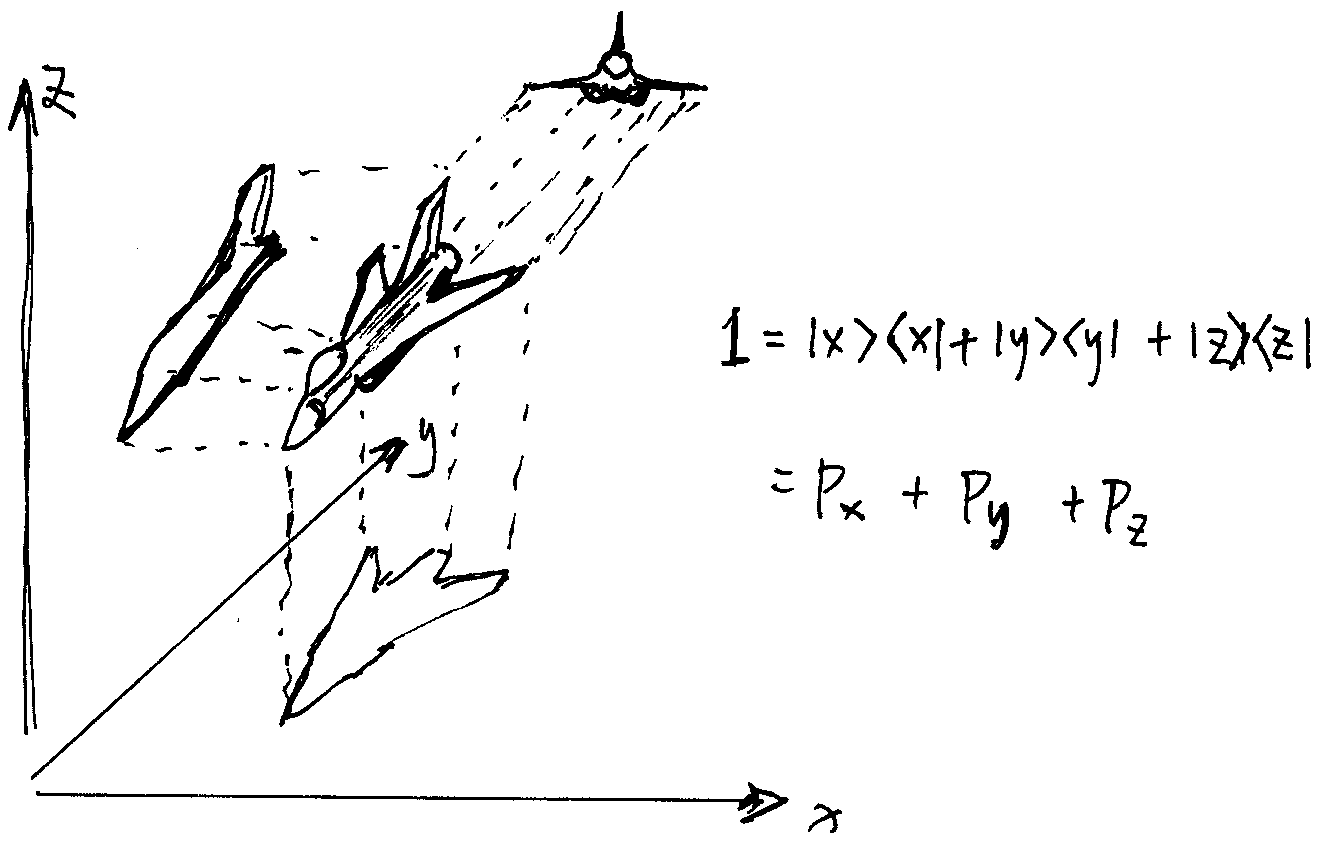
\includegraphics[width=10cm]{DiracNotation/project_to_3D.png}
\caption{三视图就是往三个方向做投影。}
%\label{default}
\end{center}
\end{figure}

同时照亮所有的面则需要很多火把,比如我们可以从两个、三个,甚至六个方向上照亮物体。假设物体是三维的,并且假设物体是“透明”的,我们需要至少从三个互相垂直的方向上照亮物体,才能获得对物体的整体认识。这个其实就是工程里的三视图,上视、侧视和前视\footnote{假如物体不是透明的那就很复杂,因为还涉及物体内部构造的问题,即便不考虑内部构造,我们也得假设物体必须是“凸起”的,才能通过六视图获得物体的整体概念。}。

光源(太阳)、物体、阴影也构成一个常见的“认识论比喻”,这就是柏拉图的“太阳喻”。我们能“看”,是因为有光,而光是源自太阳的;光照射在物体上,我们像洞穴中背对着光源的原始人一样只能看到物体的阴影,即物体本身是不对我们显现的,对我们显现的只是物体的阴影。

这里我们的兴趣并不是介绍哲学上的“太阳喻”,我们只是借助这一图像建立量子力学中的“表示概念”。

在量子力学中没有物体,只有量子态,使用狄拉克记号,记作$\left| \alpha \right\rangle$,量子态本身是无法直接被“看”到的。我们需要对量子态建立一个表示,所谓表示就是选择一个观看的方式。

以观看物体为例,就是我们拿着火把以什么样的方式把物体仔细打量一番?比如我们可以选择从$x$,$y$,$z$三个方向上照亮物体,从三个方向照亮物体其实就是把物体对这三个方向做投影。

我们把矢量$V$看做是最简单的物体,往三个方向做投影就是:

\begin{quotation}
$x$方向,方向是$e_x$,投影是$V_x = e_x \cdot V$

$y$方向,方向是$e_y$,投影是$V_y = e_y \cdot V$

$z$方向,方向是$e_z$,投影是$V_z = e_z \cdot V$
\end{quotation}

我们把量子态想象成一个矢量(态矢量,state vector),它可能有很多“方向”,每个方向都有一个单位矢量,称作基矢,记为$\left| n \right\rangle$。

在量子力学中,态矢量$\left| \alpha \right\rangle $并不直接对应观测值,在这个意义下我们也说我们是“看不见”量子态的。但我们能“看见”态矢量的投影$\left\langle n | \alpha \right\rangle $,根据玻恩的统计解释,一个量子态处在$\left| n \right\rangle$态的几率正比于$\left|  \left\langle n | \alpha \right\rangle  \right|^2 $,我们管$\left\langle n | \alpha \right\rangle$叫几率幅\footnote{我们一般只讨论已经归一化了的量子态,所以就是等于了,即量子态$\left| \alpha \right\rangle$处在$\left| n \right\rangle$态的几率等于$\left\langle n | \alpha \right\rangle^2 $。}。

我们把投影算符$P_n$定义为:$\left| n \right\rangle \left\langle n \right|$,对量子态$\left| \alpha \right\rangle$投影的效果就是获得投影$\left| n \right\rangle \left\langle n | \alpha \right\rangle$。

\begin{figure}[htbp]
\begin{center}
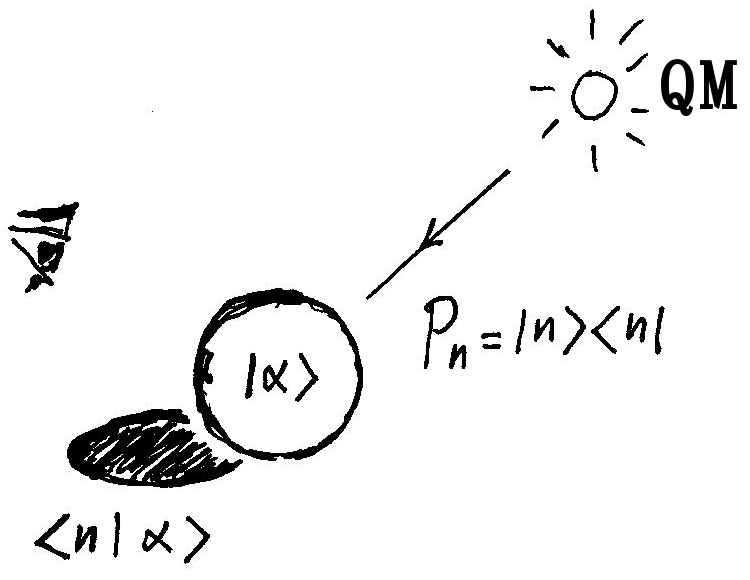
\includegraphics[width=6cm]{DiracNotation/QM_sun_interpretation.png}
\caption{一个量子力学版的“太阳比喻”}
%\label{default}
\end{center}
\end{figure}

这里基矢$\{ \left| n \right\rangle \}$的选取是关键,它决定了观看方式,我们一般是通过构造一组和哈密顿$H$两两相互都对易的算符集$\{  H, A, B, ...  \}$来构造$\{ \left| n \right\rangle \}$的。

这样几率$\left| \left\langle n | \alpha \right\rangle \right|^2 $就有了明确的物理意义:

\begin{quotation}
现在我们把$\{ \left| n \right\rangle \}$改写成$\{ \left| E_n , a, b, ... \right\rangle  \}$,几率$\left|  \left\langle E_n, a, b | \alpha \right\rangle  \right|^2 $就是量子态$\left| \alpha \right\rangle $坍缩到态$\left| E_n, a, b \right\rangle$上的几率。
\end{quotation}

\begin{table}[htdp]
\caption{太阳比喻:哲学版本和量子力学版本}
\begin{center}
\begin{tabular}{|c|c|c|}
\hline
视觉 & 哲学 & 量子力学 \\
\hline
太阳 & 善(最高理念) & 研究纲领 \\
\hline
光线 & 逻各斯(Logos) & 投影算符$P_n $ \\
物体本身 & 理念 & 量子态 $\left| \alpha \right\rangle$ \\
阴影、影像 & 现象 & 几率幅 $\left\langle n | \alpha \right\rangle$ \\
眼睛,视觉能力 & 灵魂,求知能力 & 物理学家 \\ 
\hline
\end{tabular}
\end{center}
\label{default}
\end{table}%


\subsection{狄拉克记号}

下面我们将结合自旋1/2这个例子讨论量子力学中的狄拉克记号(Dirac Notation)。在理论物理学中记号法很重要,合适的记号法会使数学推导清晰简洁并且不容易出错。

狄拉克记号就是括号,括号在英文里是:

\begin{center}
bracket
\end{center}

我们把它表示为:

\begin{equation}
\left\langle  {bra}  \right|  {c} \left|   {ket}  \right\rangle 
\end{equation}

左边括号的“尖头”是向左的,我们称$\left\langle  {  }  \right|$是左矢空间(bra space)中的一个矢量(简称“左矢”),右边的括号的“尖头”是向右的,我们称$\left|  { }  \right\rangle $是右矢空间(ket space)中的一个矢量(简称“右矢”)。左矢和右矢中间夹着一个“内容”(content),这个内容是算符(operator),我们一般用大写字母$A$表示算符。

\begin{figure}[htbp]
\begin{center}
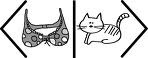
\includegraphics[width=4cm]{DiracNotation/bracket.png}
\caption{一个卡通化的“bra”和“cat”,即“胸罩”和“咪咪”。这个图对应的是“内积”。}
%\label{default}
\end{center}
\end{figure}

\subsubsection{向量、左矢和右矢}

针对自旋1/2的量子态,我们建立如下映射/表示关系:

\begin{eqnarray}
\left| + \right\rangle &\dot =& \left( \begin{array}{ccc} 1 \\ 0 \end{array} \right) \\
\left| - \right\rangle &\dot =& \left( \begin{array}{ccc} 0 \\ 1 \end{array} \right)
\end{eqnarray}

这里我们把$\left| z \pm \right\rangle$简记为$\left| \pm \right\rangle$,$\left| \pm \right\rangle$是互相排斥的同时完备的两个分类“标准”,任意的一个二维列向量$\left| \alpha \right\rangle$可以表示为它们的叠加:

\begin{equation}
\left| \alpha \right\rangle = a \left| + \right\rangle + b \left| - \right\rangle = \left( \begin{array}{ccc} a \\ b \end{array}  \right)
\end{equation}

这里的叠加系数$a$,$b$是复数(complex number)。在量子力学中我们用态矢量$\left| \alpha \right\rangle$表示系统的一个态。复数$c$是所谓对易数,它可以随便出现在列向量(态)的左边或者右边,或者我们把它和$\alpha$写在一起放在括号里面:

\begin{equation}
c \left| \alpha \right\rangle = \left| \alpha \right\rangle c = \left| c \alpha \right\rangle
\end{equation}

~

假设有两个向量$\left|  \alpha \right\rangle$、$\left| \beta \right\rangle$,我们想知道这两个向量的相似程度。如果在笛卡尔空间,我们让$\left|  \alpha \right\rangle$向$\left|  \beta \right\rangle$投影,记做:

\begin{equation}
\left|  \beta \right\rangle \left\langle \beta | \alpha  \right\rangle
\end{equation}

投影之后,向量在$\left| \beta \right\rangle$方向上,同时大小变成$\left\langle \beta | \alpha  \right\rangle$,即$\left| \alpha \right\rangle$在$\left| \beta \right\rangle$方向上的投影是$\left\langle \beta | \alpha  \right\rangle$倍的$\left| \beta \right\rangle$。

$\left\langle \beta | \alpha  \right\rangle$是个数,假如:

\begin{eqnarray*}
\left| \alpha \right\rangle &=& \left( \begin{array}{ccc} a \\ b \end{array} \right) \\
\left| \beta \right\rangle &=& \left( \begin{array}{ccc} c \\ d \end{array} \right)
\end{eqnarray*}

$\left\langle \beta | \alpha  \right\rangle$被定义为:

\begin{equation}
\left\langle \beta | \alpha  \right\rangle = \left( c^* , d^* \right) \left( \begin{array}{ccc}  a \\ b  \end{array}  \right) = c^* a + d^* b
\end{equation}

我们称$\left\langle \beta | \alpha  \right\rangle$为内积(inner product),这样定义内积的好处是会使向量$\left| \alpha \right\rangle$,自己和自己的内积——$ \left\langle \alpha | \alpha  \right\rangle $——是非负的。

\begin{equation*}
\left\langle \alpha | \alpha  \right\rangle = \left( a^* , b^* \right) \left( \begin{array}{ccc}  a \\ b  \end{array}  \right) = a^*a + b^* b \ge 0
\end{equation*}

如果向量$\left| \alpha \right\rangle$本身不是0向量,那么我们总可以把它归一化(normalized),归一化的因子是:

\begin{equation*}
\frac{1}{\sqrt { a^* a + b^* b }}
\end{equation*}

为了叙述的方便,下面我们引入几个术语(terminology):

\begin{enumerate}
\item 

$\left| \alpha \right\rangle$叫狄拉克“右矢”(ket),对每一个狄拉克右矢而言,都有一个狄拉克“左矢”(bra)与其对应,记作:$\left\langle \alpha \right|$。

\item

以二维复系数线性空间为例,一个狄拉克右矢可以表示为$\left| \alpha \right\rangle = \left( \begin{array}{ccc} a \\ b \end{array}  \right)$,与之对应的左矢$ \left\langle \alpha \right| $可表示为:$\left( a^* , b^*  \right)$。

即转置(transpose)再加复共轭(complex conjugate)。

转置的定义是:

\begin{equation}
\left( a_{ij}  \right)^T = \left( a_{ji} \right)
\end{equation}

即矩阵中“行变成列,列变成行”。比如:第一行第一列的元素,变到第一行第一列;第二行第一列的元素,变到第一行第二列。

复共轭的定义是:

\begin{equation}
\left( a_{ij}  \right)^* = \left( a_{ij}^* \right)
\end{equation}

即矩阵中每一个元素都取复共轭。

转置再加复共轭整体叫做厄米共轭(Hermite conjugate),表示为:

\begin{equation}
\left( a_{ij}  \right)^{\dagger} = \left( a_{ji}^* \right)
\end{equation}

\item

我们管$\left| \alpha \right\rangle  \leftrightarrow  \left\langle \alpha \right|$这样的关系叫“对偶”(dual correspondence),即对一个右矢而言存在一个左矢与之对应,相反对一个左矢而言也存在一个右矢与之对应。

\end{enumerate}

关于对偶,我们可以总结如下性质:

\begin{enumerate}
\item 

两向量相加的对偶:

\begin{equation}
\left| \alpha \right\rangle + \left| \beta \right\rangle  \leftrightarrow \left\langle \alpha \right| + \left\langle \beta \right|
\end{equation}

\item

复数乘一个向量的对偶:

\begin{equation}
c \left| \alpha \right\rangle  \leftrightarrow c^* \left\langle \alpha \right|
\end{equation}

\item

内积的对偶:

\begin{equation}
\left\langle \beta | \alpha \right\rangle = \left\langle \alpha | \beta \right\rangle^*
\end{equation}

\end{enumerate}

\subsubsection{算符}

算符(operator)就是操作,我们把算符定义为对矢量的操作,它把一个矢量映射为另一个矢量,比如它把一个右矢映射为另一个右矢:

\begin{equation}
A \left| \gamma \right\rangle = \left| \alpha \right\rangle \left\langle \beta |  \gamma \right\rangle =  \left\langle \beta |  \gamma \right\rangle  \left| \alpha \right\rangle = \left| \delta \right\rangle
\end{equation}

这里$ \left| \alpha \right\rangle \left\langle \beta \right| $,我们称之为两个向量的外积(outer product),就是算符$A$,它把右矢$\left|  \gamma \right\rangle$映射为$\left| \delta \right\rangle$。

\begin{equation}
A \left| \gamma \right\rangle = \left| \delta \right\rangle
\end{equation}

$\left| \delta \right\rangle$的对偶是$\left\langle  \delta \right|$,那么$A \left| \gamma \right\rangle$的对偶是什么呢?

我们把$A \left| \gamma \right\rangle$的对偶记作:

\begin{equation}
\left\langle \gamma \right| A^\dagger = \left\langle \delta \right|
\end{equation}

为了避免运算中出错,这里算符$A^\dagger$看作是向右——即对右矢——起作用的。

我们称$A^\dagger $是$A$的厄米共轭,并且$A$与$A^\dagger $互为厄米共轭。

下面我们来做几个练习:

\begin{enumerate}
\item 

$A = \left| \alpha \right\rangle \left\langle \beta \right|$,那么$A^\dagger = ?$

解:

把$A$作用于任意右矢$\left| \gamma \right\rangle$,然后求它的对偶:

\begin{equation*}
\left| \alpha \right\rangle \left\langle \beta | \gamma \right\rangle \leftrightarrow \left\langle \beta | \gamma \right\rangle^* \left\langle \alpha \right| = \left\langle \gamma | \beta \right\rangle \left\langle \alpha \right|
\end{equation*}

同时我们又有厄米共轭的定义:

\begin{equation*}
A \left| \gamma \right\rangle \leftrightarrow \left\langle \gamma \right|   A^\dagger
\end{equation*}

因此:

\begin{equation}
\left(  \left| \alpha \right\rangle \left\langle \beta \right|  \right)^\dagger = \left| \beta \right\rangle \left\langle \alpha \right|
\end{equation}


\item

定义两算符的相乘$AB $为

\begin{equation}
AB \left| \alpha \right\rangle = A \left( B \left| \alpha \right\rangle  \right)
\end{equation}

那么$AB$整体的厄米共轭$(AB)^\dagger = ?$

解:

先考虑$B$对$\left| \alpha \right\rangle$的作用$\left| \beta \right\rangle =  B \left| \alpha \right\rangle$,它的对偶是:

\begin{equation*}
\left| \beta \right\rangle = B \left| \alpha \right\rangle \leftrightarrow \left\langle \beta \right| = \left\langle \alpha \right| B^\dagger
\end{equation*}

现在考虑$AB \left| \alpha \right\rangle$的对偶:

\begin{equation*}
A B \left| \alpha \right\rangle = A \left| \beta \right\rangle \leftrightarrow \left\langle \beta \right| A^\dagger = \left\langle \alpha \right| B^\dagger A^\dagger 
\end{equation*}

同时我们又知道:

\begin{equation*}
A B \left| \alpha \right\rangle  \leftrightarrow \left\langle \alpha \right|  \left( AB \right)^\dagger 
\end{equation*}

因此:

\begin{equation}
\left(  AB \right)^\dagger = B^\dagger A^\dagger 
\end{equation}

\item

定义厄米算符为:

\begin{equation}
A^\dagger = A
\end{equation}

即:如果一个算符$A$的厄米共轭$A^\dagger $就是它自己的话,我们就说它是厄米的(Hermitian)。

证明如下等式对厄米算符成立:

\begin{equation}
\left\langle \beta \right| A \left| \alpha \right\rangle =  \left\langle \alpha \right| A \left| \beta \right\rangle^*
\end{equation}

证:

\begin{equation*}
\left\langle \beta \right| A \left| \alpha \right\rangle = \left\langle \beta \right|  \left( A \left| \alpha \right\rangle \right)  =   \{ \left(  \left\langle \alpha \right| A^\dagger \right) \left| \beta \right\rangle \}^* 
\end{equation*}

考虑到$A$是厄米的,$A^\dagger = A$:

\begin{equation*}
\left\langle \beta \right| A \left| \alpha \right\rangle = \left\langle \alpha \right| A \left| \beta \right\rangle^*
\end{equation*}

假如$\left| \beta \right\rangle = \left| \alpha \right\rangle$的话,

\begin{equation*}
\left\langle \alpha \right| A \left| \alpha \right\rangle = \left\langle \alpha \right| A \left| \alpha \right\rangle^*
\end{equation*}

一个数的复共轭就是这个数自己,这说明$\left\langle \alpha \right| A \left| \alpha \right\rangle$是个实数(real number)。

由于物理可观测量的数值必须是实数(而不能是复数),在量子态$\left| \alpha \right\rangle$下,$\left\langle \alpha \right| A \left| \alpha \right\rangle$就可以用来表示物理量A的期望值(expectation value),前提是我们必须用一个厄米算符$A$来表示物理量A。

\end{enumerate}



\subsubsection{本征值问题}

考虑:

\begin{equation}
A \left| a' \right\rangle = a' \left| a' \right\rangle
\end{equation}

即:算符作用于右矢上,其后果是这个算符自身再乘上一个复数,于是这个复数就可用来标记(命名)这个右矢。

$a'$叫做本征值(eigen value),$\left| a' \right\rangle$叫做本征矢(eigen vector),$\left| a' \right\rangle$是与$a'$对应的本征矢。把所有符合$A \left| a' \right\rangle = a' \left| a' \right\rangle$条件的$a'$及其对应的$\left| a' \right\rangle $都求出来的挑战叫做“求解本征值问题”。

我们可以证明,假如$A$是厄米算符的话,其本征值$a'$一定是实数。并且如果有两个本征值$a'$和$a''$,假如$a' \neq a''$的话,它们对应的本征矢$\left\langle a' | a'' \right\rangle = 0$,即$\left| a' \right\rangle$和$\left| a'' \right\rangle$一点都不像。

证:

由本征值问题:

\begin{equation*}
A \left| a' \right\rangle = a' \left| a' \right\rangle
\end{equation*}

出发。其对偶形式是:

\begin{equation*}
\left\langle a'' \right| A^\dagger =  \left\langle a'' \right| A = a''^* \left\langle a'' \right|
\end{equation*}

再把上式作用于右矢$\left| a' \right\rangle$

\begin{equation*}
\left\langle a'' \right| A \left| a' \right\rangle = a' \left\langle a'' | a' \right\rangle = a''^* \left\langle a'' | a' \right\rangle
\end{equation*}

整理一下:

\begin{equation*}
\left( a' - a''^* \right) \left\langle a'' | a' \right\rangle = 0
\end{equation*}

假如$a'$就是$a''$的话,只要$\left| a' \right\rangle$不是0矢量,$\left\langle a' | a' \right\rangle > 0 $,因此:

\begin{equation*}
a' = a'^*
\end{equation*}

一个数的复共轭就等于这个数自己,这意味着这个数的虚部为0,或这个数是实数。

现在假设$a' \neq a''$,同时利用刚刚证明出的结果$a'$和$a''$都是实数,考虑:

\begin{equation*}
\left( a' - a'' \right) \left\langle a''  | a'  \right\rangle = 0
\end{equation*}

因为$a' - a'' \neq 0$,内积$\left\langle a''  | a'  \right\rangle$就必须为0。

~

假设$\left| a' \right\rangle$是$A$的本征矢,任意乘一个复数,$c \left| a' \right\rangle$也是$A$的本征矢,一般我们提到的本征矢$\left| a' \right\rangle$都是归一化的本征矢。

根据以上证明,算符$A$的所有本征矢$\left| a' \right\rangle$构成一个集合$\{ \left| a' \right\rangle \}$,并且满足正交归一(orthonormal)的关系。

\begin{equation}
\left\langle a' | a'' \right\rangle = \delta_{a', a''}
\end{equation}

这里$\delta_{a', a''}$是克罗尼克记号,当$a' = a''$时,$\left| a' \right\rangle$是归一的,即$\delta_{a', a''} = 1$;当$a' \neq a''$时,$\left| a' \right\rangle$和$\left| a'' \right\rangle$是正交的,即$\delta_{a', a''} = 0$。

~

这里我们忽略了一种情况,即一个本征值$a'$,它有可能对应多个不同的本征矢量,比如$\left| a'_1 \right\rangle $、$\left| a'_2 \right\rangle $……$\left| a'_f \right\rangle$。一个本征值和$f$个不同的本征矢量对应,我们称这种情况为简并,简并度为$f$。

对于存在简并的本征值问题,原则上我们也能得到一个正交归一的本征矢的集合$\{ \left| a' \right\rangle \}$,难的是给它们起名字,或做标记。

因为一个$a'$有可能对应好几个不同的$\left| a'_1 \right\rangle $、$\left| a'_2 \right\rangle $、……,仅仅靠$a'$我们是无法分辨它们的。

这就要求我们考虑新的本征值问题。比如,考虑算符$B$的本征值问题,为了使$B$及其对应的分类命名体系在物理上有意义,我们要求$B$也是个厄米算符。

假设$A$和$B$是对易的,即

\begin{equation}
AB = BA
\end{equation}

$A$的本征值问题存在简并,即存在某个本征值$a'$,有$\left| a'_1 \right\rangle$,$\left| a'_2 \right\rangle$,……,$\left| a'_f \right\rangle$,$f$个不同的本征矢与$a'$对应,现在的关键是找到给它们标记的方案,光靠$A$的本征值$a'$是不够的。

首先,对$i = 1, 2,... f$,我们有:

\begin{equation}
A \left| a'_i \right\rangle = a' \left| a'_i \right\rangle 
\end{equation}

我们定义这$f$个不同的本征矢的线性叠加$\left| \alpha \right\rangle $:

\begin{equation}
\left| \alpha \right\rangle = \sum\limits_i c_i \left| a'_i \right\rangle
\end{equation}

对$\left| \alpha \right\rangle $,我们依然有:

\begin{equation}
A \left| \alpha \right\rangle  = a' \left| \alpha \right\rangle
\end{equation}

考虑到$A$,$B$对易:

\begin{equation}
AB \left| \alpha \right\rangle = B A \left| \alpha \right\rangle = a' B \left| \alpha \right\rangle
\end{equation}

上式中最左边的一项和最右边的一项说明$B \left| \alpha \right\rangle $依然是$A$的本征矢。

假设算符$B$满足关系:$B \left| \alpha \right\rangle = b' \left| \alpha \right\rangle$,求解本征值问题:

\begin{equation}
B \left| \alpha \right\rangle = b' \left| \alpha \right\rangle
\end{equation}

$\left| \alpha \right\rangle$可以表示为一个$f$维的列向量。

\begin{equation}
\left| \alpha \right\rangle \dot = \left( \begin{array}{ccc} c_1 \\ c_2 \\ ... \\ c_f  \end{array} \right)
\end{equation}

我们需要求解的线性代数问题是:

\begin{equation}
\left( B - b' I \right) \left( \begin{array}{ccc} c_1 \\ c_2 \\ ... \\ c_f  \end{array} \right)  = 0
\end{equation}

如果我们要求关于$\left( \begin{array}{ccc} c_1 \\ c_2 \\ ... \\ c_f  \end{array} \right)$的非零解,我们就得要求如下行列式为0:

\begin{equation}
\det \left( B - b' I \right) = 0
\end{equation}

这是一个关于$b'$的一元$f$次方程。

幸运的话,我们能求出$f$个不同的$b'$的取值,$b'_1, b'_2, ... b'_f$。把$b'$值代回方程我们能得到不同的本征矢,记作$\left| a', b'_i \right\rangle$,$i = 1, 2, ...f$。

~

我们一般会笼统地把$A$,$B$的共同本征态记作$\left| a', b' \right\rangle$,

%但也可能求不出$f$个不同的$b'$,我们可以笼统地把$A$,$B$的共同本征态记作$\left| a', b' \right\rangle$,

%存在$A$,$B$的共同本征态$\left| a', b' \right\rangle$使得:

\begin{eqnarray}
A \left| a', b' \right\rangle &=& a' \left| a', b' \right\rangle \\
B \left| a', b' \right\rangle &=& b' \left| a', b' \right\rangle
\end{eqnarray}

在引入新的指标$b'$后,$a', b'$在一起就有可能把简并消除掉,即不同的本征矢$\{  \left| a', b' \right\rangle  \}$可以和指标$\{ a', b' \}$构成“一一对应”。

如果还存在简并的话,原则上我们可以引入更多两两都对易的厄米算符的集合;由于在量子力学中我们用厄米算符表示物理量,我们也说找到一个“两两都对易的力学量(或物理量)的集合”,$\left( H, A, B, ...  \right)$。

这里总会包括哈密顿算符$H$,因为哈密顿算符对应能量,在物理里我们最关心能量,比如对求解氢原子的量子力学问题,我们会取这样一个两两都对易的力学量的集合$\left( H, L^2, L_z  \right)$。

$H$对应的是主量子数$n$,对应的本征值问题是:

\begin{equation}
H \left| n \right\rangle = E_n \left| n \right\rangle 
\end{equation}

$L^2$是轨道角动量算符的平方,$L_z$是轨道角动量算符在$z$方向上的分量,对应的本征值问题是:

\begin{eqnarray}
L^2 \left| l, m \right\rangle & = & l (l + 1 )\hbar^2 \left| l, m \right\rangle \\
L_z \left| l, m \right\rangle & = & m \hbar \left| l, m \right\rangle
\end{eqnarray}

$n, l, m$一起构成了对氢原子量子态$\left| n, l, m \right\rangle$进行描述的恰当语言。(所谓恰当就是分类的合理,每个不同的对象都有命名,而命名和命名之间有绝不重复)

所有的$\left| n, l, m \right\rangle$,两两都是正交归一的:

\begin{equation}
\left\langle n', l', m' | n, l, m \right\rangle = \delta_{nn'} \delta_{ll'} \delta_{mm'}
\end{equation}

它们的集合$\{ \left| n, l, m \right\rangle \}$构成了基矢(basisi),任意用$H$描述的物理系统的量子态可以表示为$\{ \left| n, l, m \right\rangle \}$的线性叠加。

\subsubsection{投影算符}

假设$\{  \left| n \right\rangle \}$构成基矢,基矢就相当于笛卡尔坐标系里的$\{ i, j, k \}$

笛卡尔坐标系里的任意向量$V$可以表示为向$i$($x$方向的单位矢量),$j$($y$方向的单位矢量),$k$($z$方向的单位矢量)三个方向的投影之和。

\begin{equation}
V = i V_x + j V_y + k V_z
\end{equation}

这里$V_x$是$V$向$i$的投影,表示为$V \cdot i$,我们也可以把它们按照狄拉克记号的形式进行改写:

\begin{equation}
\left| V \right\rangle =\left| i \right\rangle \left\langle i | V \right\rangle + \left| j \right\rangle \left\langle j | V \right\rangle + \left| k \right\rangle \left\langle k | V \right\rangle
\end{equation}

这里的$\left| i \right\rangle \left\langle i \right|$,$\left| j \right\rangle \left\langle j \right|$和$\left| k \right\rangle \left\langle k \right|$就是投影算符,分别表示把向量$\left| V \right\rangle $向$\left| i \right\rangle $,$\left| j \right\rangle $或$\left| k \right\rangle $投影的动作。

向所有方向投影再加起来就是单位算符$I$

\begin{equation}
I = \left| i \right\rangle \left\langle i \right| + \left| j \right\rangle \left\langle j \right| + \left| k \right\rangle \left\langle k \right|
\end{equation}

对量子力学而言,我们的基矢是$\left| n \right\rangle $,投影算符$P_n$是:

\begin{equation}
P_n = \left| n \right\rangle \left\langle n \right|
\end{equation}

表示向第$n$个基矢$\left| n \right\rangle$的投影动作。

单位算符是:

\begin{equation}
I = \sum\limits_n \left| n \right\rangle \left\langle n \right|
\end{equation}

这个表达式是量子力学中最重要的公式,因为我们可以选择不同的分类体系(其实就是表象),这样我们就可以让物理陈述在不同的表象间变换。

\subsubsection{幺正算符}

考虑一个已经被归一化了的量子态$\alpha$,

\begin{equation}
\left\langle \alpha | \alpha \right\rangle = 1
\end{equation}

假设态可以经历一个变化,这个变化用算符$U$表示,它使得:

\begin{eqnarray*}
\left| \alpha \right\rangle & \to & U \left| \alpha \right\rangle \\
\left\langle \alpha \right| & \to & \left\langle \alpha \right| U^\dagger
\end{eqnarray*}

假设我们考虑的物理过程$U$不会导致粒子的产生和湮灭,即:

\begin{equation}
\left\langle \alpha | \alpha \right\rangle \to  \left\langle \alpha \right| U^\dagger U \left| \alpha \right\rangle = 1
\end{equation}

这意味着$U$满足:

\begin{equation}
U^\dagger U = I
\end{equation}

这里$I$表示单位算符,但我们往往也把单位算符就简单地写作1,实际上在进行推导的时候,必要的简略是不可避免的,甚至如何简略公式的表达本来就是物理思维的一部分。

满足关系$U^\dagger U = 1$的算符$U$是幺正算符(Unitary operator),一般来说幺正算符不是厄米算符。

%并不仅仅是厄米算符才在量子力学中有用。

\subsection{自旋的泡利矩阵表示}

回到自旋1/2的例子,我们定义自旋算符$S$为

\begin{equation}
S = i S_x + j S_y + k S_z
\end{equation}

这里的$S_z$是自旋算符在$z$方向上的分量,它可定义为:

\begin{equation}
S_z = \frac{\hbar}{2} \left( \left| + \right\rangle \left\langle + \right| - \left| - \right\rangle \left\langle - \right|  \right)
\end{equation}

它使得:

\begin{eqnarray}
S_z \left| + \right\rangle &=& \frac{\hbar}{2} \left| + \right\rangle \\
S_z \left| - \right\rangle &=& - \frac{\hbar}{2} \left| - \right\rangle
\end{eqnarray}

这对应$z$方向的非均匀磁场(SGz)可以把“非极化”的Ag原子束分裂为相等percentage的上下两束。

我们还可以写出$S_z$的矩阵表示:

\begin{equation}
S_z =  \frac{\hbar}{2} \left( \begin{array}{ccc}  1 & 0 \\ 0 & 1   \end{array}  \right)
\end{equation}

~

我们把$S_x$定义为:

\begin{equation}
S_x = \frac{\hbar}{2} \left( \left| x+ \right\rangle \left\langle x+ \right| - \left| x- \right\rangle \left\langle x- \right| \right)
\end{equation}

这意味着$x$方向的非均匀磁场(SGx)可以把“非极化”的Ag原子束分裂为相等percentage的“左右”两束。

我们一般取$\left| z+ \right\rangle = \left| + \right\rangle = \left( \begin{array}{ccc} 1 \\ 0 \end{array} \right)  $,$\left| z- \right\rangle = \left| + \right\rangle = \left( \begin{array}{ccc} 0 \\ 1 \end{array} \right)  $,这种对基矢的取法叫$S_z$表象。这意味着$S_x$的矩阵表示就不能是对角的了。

我们可以这么来计算$S_x$的矩阵表示:

\begin{equation}
S_x \dot = \left( \begin{array}{ccc}  \left\langle + \right| S_x \left| + \right\rangle  &  \left\langle + \right| S_x \left| - \right\rangle \\   \left\langle - \right| S_x \left| + \right\rangle  &   \left\langle - \right| S_x \left| - \right\rangle  \end{array} \right) 
\end{equation}

利用:

\begin{eqnarray*}
\left| x+ \right\rangle  & = & \frac{1}{\sqrt{2}} \left(  \begin{array}{ccc} 1 \\ 1  \end{array} \right) \\
\left| x- \right\rangle & = &  \frac{1}{\sqrt{2}} \left(  \begin{array}{ccc} -1 \\ 1  \end{array} \right)
\end{eqnarray*}

我们可以计算比如矩阵中的第一项:

\begin{eqnarray*}
\left\langle + \right| S_x \left| + \right\rangle &=& \frac{\hbar}{2} \left( \left\langle + | x+ \right\rangle \left\langle x+ | + \right\rangle - \left\langle + | x- \right\rangle \left\langle x- | + \right\rangle   \right) \\
{} &=& \frac{\hbar}{2} \left( \frac{1}{2} - \frac{1}{2} \right) = 0
\end{eqnarray*}

最终计算出$S_x$的矩阵表示是:

\begin{equation}
S_x  = \frac{\hbar}{2} \left( \begin{array}{ccc} 0 &  1 \\ 1 & 0 \end{array} \right)
\end{equation}

~

我们把$S_y$定义为:

\begin{equation}
S_y = \frac{\hbar}{2} \left( \left| y+ \right\rangle \left\langle y+ \right| - \left| y- \right\rangle \left\langle y- \right| \right)
\end{equation}

其矩阵表示为:

\begin{equation}
S_y \dot = \left( \begin{array}{ccc}  \left\langle + \right| S_y \left| + \right\rangle  &  \left\langle + \right| S_y \left| - \right\rangle \\   \left\langle - \right| S_y \left| + \right\rangle  &   \left\langle - \right| S_y \left| - \right\rangle  \end{array} \right) = \frac{\hbar}{2} \left( \begin{array}{ccc} 0 &  -i \\ i & 0 \end{array} \right) 
\end{equation}

小结一下:

\begin{eqnarray}
S_x &=& \frac{\hbar}{2} \sigma_x =  \frac{\hbar}{2} \left( \begin{array}{ccc} 0 &  1 \\ 1 & 0 \end{array} \right)  \\
S_y &=& \frac{\hbar}{2} \sigma_y = \frac{\hbar}{2} \left( \begin{array}{ccc} 0 &  -i \\ i & 0 \end{array} \right)  \\
S_z &=& \frac{\hbar}{2} \sigma_z = \frac{\hbar}{2} \left( \begin{array}{ccc} 1 &  0 \\ 0 & -1 \end{array} \right)  
\end{eqnarray}

这里$\sigma_x = \left( \begin{array}{ccc} 0 &  1 \\ 1 & 0 \end{array} \right) $,$\sigma_y = \left( \begin{array}{ccc} 0 &  -i \\ i & 0 \end{array} \right) $,$\sigma_z = \left( \begin{array}{ccc} 1 &  0 \\ 0 & -1 \end{array} \right) $。再加上单位矩阵$I =  \left( \begin{array}{ccc} 1 &  0 \\ 0 & 1 \end{array} \right)$,总共四个合称泡利矩阵(Pauli matrices)。

%任意一个$2 \times 2$的厄米矩阵都可以表示为以上四个泡利矩阵的线性叠加。

%这是因为一个$2 \times 2$的厄米矩阵可表示为:

%\begin{equation}
%\left( \begin{array}{ccc}  a  & c+ id  \\  c- i d & b  \end{array} %\right)
%\end{equation}

%这里$a, b, c, d$都是实数,正好对应四个独立的变量。

~

我们可以验证自旋$S$确实符合角动量的性质:

\begin{eqnarray}
\left[ S_x , S_y  \right]  & = & i \hbar S_z\\
\left[ S_y , S_z  \right]  & = & i \hbar S_x\\
\left[ S_z , S_x  \right]  & = & i \hbar S_y\\
\left[S_x , S^2 \right] & = & \left[S_y , S^2 \right] = \left[S_z , S^2 \right] =  0
\end{eqnarray}

~

升降算符$S^+$和$S^-$可以大大简化涉及自旋算符的量子力学计算:

%我们定义升降算符$S^+$和$S^-$为:

\begin{eqnarray}
S^+ & = & \hbar  \left| + \right\rangle \left\langle - \right|  \\
S^- & = & \hbar  \left| - \right\rangle \left\langle + \right|
\end{eqnarray}

$S^+$的作用是使$\left| - \right\rangle$ 变成 $\left| + \right\rangle$,

\begin{equation}
S^+ \left| - \right\rangle = \hbar  \left| + \right\rangle \left\langle -  | -   \right\rangle = \hbar \left| + \right\rangle
\end{equation}

$S^-$的作用是使$\left| + \right\rangle$ 变成 $\left| - \right\rangle$,

\begin{equation}
S^- \left| + \right\rangle = \hbar  \left| - \right\rangle \left\langle +  | +   \right\rangle = \hbar \left| - \right\rangle
\end{equation}

升降算符是极形象的命名。

我们可以把“升降算符”表示为一个$2 \times 2$的方阵,它使得一个“$2 \times 2$的方阵”乘以一个“二维列向量”等于一个“二维列向量”,这就是算符的“矩阵表示”。

比如$S^+$的矩阵表示是:

\begin{equation}
S^+ \dot = \left(  \begin{array}{ccc}  S^+_{++} &  S^+_{+-} \\  S^+_{-+} & S^+_{--}  \end{array} \right)
\end{equation}

这里的矩阵元分别是:

\begin{eqnarray*}
S^+_{++} &=& \left\langle + \right| S^+ \left| + \right\rangle = \hbar \left\langle + | +  \right\rangle  \left\langle  - | + \right\rangle = 0 \\
S^+_{+-} &=&  \left\langle + \right| S^+ \left| - \right\rangle = \hbar \left\langle + | + \right\rangle  \left\langle - | - \right\rangle = 1 \\
S^+_{-+} &=& \left\langle - \right| S^+ \left| + \right\rangle = \hbar \left\langle - | + \right\rangle \left\langle - | + \right\rangle = 0 \\
S^+_{--} &=&  \left\langle - \right| S^+ \left| - \right\rangle = \hbar \left\langle - | + \right\rangle \left\langle - | - \right\rangle = 0
\end{eqnarray*}

这里我们利用了:

\begin{eqnarray*}
\left\langle + | + \right\rangle & = & \left\langle - | - \right\rangle = 1 \\
\left\langle + | - \right\rangle & = & \left\langle - | + \right\rangle = 0
\end{eqnarray*}

因此,自旋1/2的升算符$S^+$可表示为:

\begin{equation}
S^+ \dot = \hbar \left(  \begin{array}{ccc}  0 &  1 \\  0 & 0  \end{array} \right)
\end{equation}

类似地,可求出降算符$S^-$的矩阵表示(或直接利用性质:$\left( S^+ \right)^\dagger = S^-$):

\begin{equation}
S^- \dot = \hbar \left(  \begin{array}{ccc}  0 &  0 \\  1 & 0  \end{array} \right)
\end{equation}

最后,我们可以验证:

\begin{equation}
S^{\pm} = S_x \pm i S_y
\end{equation}

\subsection{角动量的代数解法}

我们现在来求解$(L^2, L_z)$的共同本征值问题,通常来说这需要我们求解一个关于极角$\theta$和方位角$\phi$的偏微分方程,这是极啰嗦的,但我们也可由对易式出发,仅凭代数关系就把$(L^2, L_z)$的共同本征值问题求出来,而且我们发现在这个代数解法中,$l = 1/2$这样的解不再是不允许的了\footnote{由于代数解法中根本就不出现$\theta$和$\phi$,所以$l= 1/2$这样的解就是允许的。},这实际上给出了一个关于轨道角动量(量子数取整数)和自旋角动量(量子数取1/2)的共同描述。

假设$(L^2, L_z)$的共同本征态是$\left| \lambda, \mu  \right\rangle$,

\begin{eqnarray}
L^2 \left| \lambda, \mu \right\rangle &=& \lambda \hbar^2 \left| \lambda, \mu  \right\rangle \\
L_z \left| \lambda, \mu  \right\rangle &=& \mu \hbar \left| \lambda, \mu  \right\rangle
\end{eqnarray}


首先我们模仿自旋1/2的情形定义升降算符$L^{\pm}$:

\begin{eqnarray}
L^+ &=& L_x + i L_y  \\
L^- &=& L_x - i L_y 
\end{eqnarray}

我们可以证明对易式:

\begin{equation*}
[ L_z, L^+ ] = [L_z, L_x + i L_y] = L_z L^+ - L^+ L_z = \hbar L^+
\end{equation*}

利用:

\begin{equation*}
( L_z L^+ - L^+ L_z ) \left| \lambda, \mu  \right\rangle = \hbar L^+ \left| \lambda, \mu \right\rangle
\end{equation*}

考虑到:$L^+ L_z \left| \lambda, \mu \right\rangle = \mu \hbar L^+ \left| \lambda, \mu \right\rangle $,

\begin{equation}
L_z L^+ \left| \lambda, \mu \right\rangle = (\mu + 1) \hbar L^+ \left| \lambda, \mu \right\rangle
\end{equation}

这里我们把$L^+ \left| \lambda, \mu \right\rangle$看成是一个新的态矢量,它也是$L_z$的本征矢,本征值为$( \mu + 1 ) \hbar$,因此$L^+ \left| \lambda, \mu \right\rangle$可表示为:

\begin{equation}
L^+ \left| \lambda, \mu \right\rangle = C \left| \lambda, \mu+1 \right\rangle
\end{equation}

这里$C$是待定的复数因子。

即$L^+$可以使量子数$\mu+1$,我们形象地称之为升算符。类似地,我们可证明$L^- \left| \lambda, \mu \right\rangle $也是$L_z$的本征矢,对应本征值为$(\mu-1) \hbar$。

因此,$L^- \left| \lambda, \mu \right\rangle$可表示为:

\begin{equation}
L^- \left| \lambda, \mu \right\rangle = C' \left| \lambda, \mu-1 \right\rangle
\end{equation}

这里$C'$是待定的复数因子。

即$L^-$可以使量子数$\mu-1$,我们形象地称之为降算符。

现在的问题是这种“升、降”操作是否可无限制地进行下去?

如果可以的话,就意味着$L_z$的本征值的大小就没有限制了,而这是不可能的。因为$L_z$仅仅是$L = i L_x + j L_y + k L_z$算符的一个分量,而我们假设$L^2 = L_x^2 + L_y^2 + L_z^2$的本征值是$\lambda \hbar^2$,这样“升、降”操作就不能无限制地进行下去。

通俗地说就是我们假设角动量量子数是$l$,那么$\mu$的取值最大将只是$l$,再大是不可能的。

我们把这句话翻译成数学的语言,对态$\left| \lambda, l \right\rangle$,必须有:

\begin{equation}
L^+ \left| \lambda, l \right\rangle = 0
\end{equation}

对零矢量前面再乘一个算符$L^-$并不会改变计算结果,即:

\begin{equation}
L^- L^+ \left| \lambda, l \right\rangle = 0 
\end{equation}

我们把$L^- L^+$展开:

\begin{eqnarray*}
L^- L^+ &=& ( L_x - i L_y ) (L_x + i L_y) = L_x^2 + L_y^2 + i [ L_x, L_y ] \\
{} &=& L^2 - L_z^2 - \hbar L_z
\end{eqnarray*}

即:

\begin{equation}
L^2 \left| \lambda, l \right\rangle = (L_z^2 + \hbar L_z) \left| \lambda, l \right\rangle = l (l + 1)\hbar^2 \left| \lambda, l \right\rangle
\end{equation}

现在我们重新把$\lambda$写作$l (l +1)$,$\mu$重新写作$m$,$\left|  \lambda, \mu \right\rangle$写作$\left| l, m \right\rangle$,得到:

\begin{eqnarray}
L^2 \left| l,m \right\rangle &=& l(l+1)\hbar^2 \left| l,m \right\rangle \\
L_z \left| l,m \right\rangle &=& m \hbar \left| l,m \right\rangle
\end{eqnarray}

这里$m$的取值是从$l$开始逐渐“减1”,“减1”,最后得到对称的$-l$,或者我们由$-l$开始逐渐“加1”,“加1”,最后得到$l$。要得到这种结构,$l$取整数$0, 1, 2 ...$是可以的,取半整数$1/2, 3/2, ...$也是可以的,但取其他情况就不可以了。

小结一下:

\begin{eqnarray*}
l &=& 0, 1/2, 1, 3/2, 2, ...\\
m &=& l, l-1, ..., -l +1 , -l
\end{eqnarray*}

对轨道角动量而言$l$只能取整数,是我们这里讨论的一种特殊情况。

~

下面我们继续证明一个有用的性质,对升降算符$L^{\pm}$,有:

\begin{equation*}
L^{\pm} \left| l,m \right\rangle = \hbar \sqrt{(l \mp m)(l \pm m +1)
} \left|l, m \pm 1 \right\rangle
\end{equation*}

定义: $\left| \gamma \right\rangle = L^+ \left| lm
\right\rangle$, 对应到左矢空间, $\left\langle \gamma \right| =
\left\langle lm  \right| L^-$,

因此:

\begin{equation*}
\left\langle \gamma | \gamma \right\rangle = \left\langle lm \right|
L^- L^+ \left| lm \right\rangle
\end{equation*}

上式中的$L^- L^+$展开是:

\begin{equation*}
(L_x-iL_y) (L_x + i L_y) = L_x^2 + L_y^2 +i [L_x, L_y] = L^2 - L_z^2
- \hbar L_z
\end{equation*}

因此:

\begin{equation*}
\left\langle \gamma | \gamma \right\rangle = \left\langle L^2 -
L_z^2 - \hbar L_z \right\rangle = l(l+1)\hbar^2 - m^2\hbar^2 -m
\hbar^2
\end{equation*}

上式化简可得:

\begin{equation*}
\left\langle \gamma | \gamma \right\rangle =  (l - m)(l+m+1)\hbar^2
\end{equation*}

即:

\begin{equation}
L^+  \left| l, m \right\rangle = \hbar \sqrt{(l - m)(l + m +1) } \left|l, m + 1 \right\rangle
\end{equation}

类似地,我们还可对降算符$L^-$证明:

\begin{equation}
L^-  \left| l, m \right\rangle = \hbar \sqrt{(l + m)(l - m +1) } \left|l, m - 1 \right\rangle
\end{equation}

\subsection{自旋单态和自旋三重态}

假设有两个自旋,自旋甲和自旋乙,它们是独立的,所谓独立就是说甲的态不会影响乙,反过来乙的态也不会影响甲。但我们现在考虑的系统是“甲和乙”。对这样“甲和乙”的自旋的态我们应如何描述。

但考虑自旋甲的话,自旋甲可以是随便一个态$\left| \alpha \right\rangle$,如果我们使用$S_z$表象的话,我们取自旋甲在$z$方向向上和向下的态$\{ \left| + \right\rangle, \left| - \right\rangle,   \}$为基矢。如此我们“张”成一个二维的线性空间,所谓“张”是个很形象的动作,好比我们在雨季撑开一把伞,$\left| + \right\rangle$和$\left| - \right\rangle$是两个互相正交归一的态,即:

\begin{eqnarray*}
\left\langle + | + \right\rangle  &=& \left\langle - | - \right\rangle  = 1\\
\left\langle + | - \right\rangle &=& \left\langle - | + \right\rangle = 0
\end{eqnarray*}

这两个互相正交归一的态矢量“像”笛卡尔坐标系中的$\vec e_x$和$\vec e_y$一样成为表示任意矢量的“一套单位向量。”

但我们要注意以上所有陈述都是针对自旋甲而言的,我们应该在记号里予以明确的说明或规定,比如我们在右下角标个指标“1”,像这样:

\begin{equation*}
\left| \alpha \right\rangle_1 = \left( \begin{array}{ccc} a \\ b \end{array} \right)_1 = a \left| + \right\rangle_1 + b \left| - \right\rangle_1
\end{equation*}

我们还有自旋乙,用完全类似的方案把它表示出来。单考虑自旋乙,任意态$\left| \beta \right\rangle_2$——这里用指标“2”表示自旋乙——可表示为:

\begin{equation*}
\left| \beta \right\rangle_2 = \left( \begin{array}{ccc} c \\ d \end{array} \right)_2 = c \left| + \right\rangle_2 + d \left| - \right\rangle_2
\end{equation*}

“甲和乙”一起考虑,我们首先要找到描述“甲和乙”的基矢,既然甲和乙是独立的,一种自然的选择是:

\begin{eqnarray}
\left| ++ \right\rangle & = & \left| + \right\rangle_1 \left| + \right\rangle_2  \\
\left| +- \right\rangle & = & \left| + \right\rangle_1 \left| - \right\rangle_2  \\
\left| -+ \right\rangle & = & \left| - \right\rangle_1 \left| + \right\rangle_2  \\
\left| -- \right\rangle & = & \left| - \right\rangle_1 \left| - \right\rangle_2 
\end{eqnarray}

这里的规则是把甲、乙两个自旋的态并列,我们规定左边的那个是甲,右边的那个是乙。总共得到四个基矢$\{ \left| ++ \right\rangle, \left| +- \right\rangle, \left| -+ \right\rangle, \left| - - \right\rangle \}$,我们可以验证这四个基矢也是两两正交归一的,比如:

\begin{eqnarray*}
\left\langle ++ | ++ \right\rangle &=& \left\langle -- | -- \right\rangle = 1 \\
\left\langle ++ | -- \right\rangle &=& \left\langle ++ | +- \right\rangle = 0 \\
{} & ... & {}
\end{eqnarray*}

这样我们就得到了直接乘积(direct product)表示,即对“甲和乙”这个系统里的任意态矢量$\left| \alpha \right\rangle$,我们可以把它表示为:

\begin{eqnarray*}
\left| \alpha \right\rangle &=& \left( \left| {++} \right\rangle \left\langle {++}  \right|  + \left| {+-} \right\rangle \left\langle {+-}  \right| + \left| {-+} \right\rangle \left\langle {-+} \right| + \left| {--} \right\rangle \left\langle {--}  \right|  \right) \left| \alpha \right\rangle \\
{} &=& a \left| {++} \right\rangle + b \left| {+-} \right\rangle + c \left| {-+} \right\rangle + d \left| {--} \right\rangle
\end{eqnarray*}

这里$I = \left( \left| {++} \right\rangle \left\langle {++}  \right|  + \left| {+-} \right\rangle \left\langle {+-}  \right| + \left| {-+} \right\rangle \left\langle {-+}  \right| + \left| {--} \right\rangle \left\langle {--}  \right|  \right)$是单位算符,它的意思是向所有方向做投影。$a, b, c, d$是投影(或几率幅):

\begin{eqnarray*}
a &=& \left\langle {++} | \alpha \right\rangle \\
b &=& \left\langle {+-} | \alpha \right\rangle \\
c &=& \left\langle {-+} | \alpha \right\rangle \\
d &=& \left\langle {--} | \alpha \right\rangle
\end{eqnarray*}

态矢量$\left| \alpha \right\rangle$所在的空间叫直接乘积空间(direct product space)\footnote{我们现在来描述什么是直积空间$C = A \otimes B$:

\begin{quote}
$A$是一个希尔伯特空间, $A=\{a_1, a_2, a_3, ...., a_i, ...\}$,
$a_i$是$A$中任一元素; 同样$B$是另外一个希尔伯特空间, $B=\{b_1, b_2,
b_3, ..., b_j, ...\}$, $b_j$是$B$中任一元素, 我们把$a_i$,
$b_j$并列地放在一起, $a_i b_j$构成了希尔伯特空间$C$中的任一元素, $C
= \{a_1b_1, a_1b_2, a_1b_3, ..., a_ib_j, ...\}$。
\end{quote}

容易证明:

\begin{enumerate}
  \item 如果$A$中有$m$个元素, $B$中有$n$个元素, 则$C$中有$m \times
n$个元素。
  \item 如果$A$是个$m$维的希尔伯特空间, 基矢是$\{a_i\}, i=1,2,...,m$,
$B$是个$n$维的希尔伯特空间, 基矢是$\{b_j\}, j=1,2,...,n$,
则$C$是个$m \times n$维的希尔伯特空间, 基矢是$\{a_ib_j\},
i=1,2,...,m; j=1,2,...,n$。
\end{enumerate}}。

这样描述有什么“物理意义”吗?或我们可以把什么样的物理量和$\{ \left| ++ \right\rangle, \left| +- \right\rangle, \left| -+ \right\rangle, \left| -- \right\rangle \}$相对应?

对第一个态$\left| ++ \right\rangle$我们可以立刻猜测它描述的是总自旋为1和总自旋的$z$分量为1的态。类似地,对第四个态$\left| -- \right\rangle $我们猜测它描述的是总自旋为$-1$和总自旋的$z$分量为1的态。

当然,我们需要先定义总自旋。

我们把总自旋定义为:

\begin{equation}
S= S_1 + S_2
\end{equation}

这看起来是个很好的定义,但仔细想想并不确切,因为$S_1$只作用于自旋甲,而$S_2$只作用于自旋乙,$S_1$和$S_2$并不是一类的东西,如何相加?

对这个质疑的修正,也很简单,我们分布把$S_1$和$S_2$改写为:

\begin{eqnarray*}
S_1 & \to & S_1 \otimes  I_2 \\
S_2 & \to & I_1 \otimes S_2
\end{eqnarray*}

这样总自旋$S$就是:

\begin{equation}
S= S_1 \otimes I_2 +  I_1 \otimes S_2
\end{equation}

容易验证对总自旋$S$的分量(虽然我们没写矢量符号,但这里$S$是矢量算符),$S_x, S_y, S_z$,及$S^2 = S_x^2 + S_y^2 + S_z^2$满足角动量算符的对易关系:

\begin{eqnarray}
\left[ S_x, S_y \right] & = & i \hbar S_z \\
\left[ S_z , S^2 \right] & = & 0
\end{eqnarray}

这意味着总自旋及总自旋的$z$分量有良好的定义。

我们现在来验证对$\left| ++ \right\rangle$而言,它确实是总自旋平方和总自旋$z$分量的共同本征态。

比如对总自旋的$z$分量,我们把它重新改写为$S_z^t$

\begin{equation}
S_z^t = S_z^1 + S_z^2
\end{equation}

这里$S_z^1$和$S_z^2$严格来说也要写成直接乘积的形式,但为了书写的简洁,我们规定指标“1”只对自旋甲的态作用,而指标“2”只对自旋乙的态作用。

\begin{equation}
S_z^t \left| ++ \right\rangle = \left( S_z^1 + S_z^2 \right) \left| ++ \right\rangle = \hbar \left| ++ \right\rangle
\end{equation}

现在来考虑$S_t^2$,

\begin{equation*}
S_t^2 = \left( S_1 + S_2 \right)^2 = S_1^2 + S_2^2 + 2 S_1 \cdot S_2
\end{equation*}

这里$S_1^2$(即$S_1^2 \otimes I_2 $)和$S_2^2$(即$I_1 \otimes S_2^2$)对$\left| ++ \right\rangle$作用的结果都是$\frac{3}{4} \hbar^2 \left| ++ \right\rangle $,加起来就是$\frac{3}{2} \hbar^2 \left| ++ \right\rangle  $。

现在考虑,

\begin{equation}
S_1 \cdot S_2 = S_1^x  S_2^x + S_1^y S_2^y + S_1^z S_2^z
\end{equation}

对上式而言,最后一项$S_1^z S_2^z$很容易计算,只要记住指标“1”对甲自旋作用,指标“2”对乙自旋作用:

\begin{equation*}
S_1^z S_2^z \left| ++ \right\rangle = \frac{\hbar^2}{4} \left| ++ \right\rangle 
\end{equation*}

前两项$S_1^x S_2^x + S_1^y S_2^y$不太好处理,但我们可以利用升降算符的定义予以改写:

\begin{eqnarray*}
S_1^+ &=& S_1^x + i S_1^y \\
S_2^- &=& S_2^x - i S_2^y \\
S_1^+ S_2^- &=& S_1^x S_2^x + S_1^y S_2^y + i S_1^y S_2^x - i S_1^x S_2^y
\end{eqnarray*}

类似地:

\begin{eqnarray*}
S_1^- &=& S_1^x - i S_1^y \\
S_2^+ &=& S_2^x + i S_2^y \\
S_1^- S_2^+ &=& S_1^x S_2^x + S_1^y S_2^y - i S_1^y S_2^x + i S_1^x S_2^y
\end{eqnarray*}

把上面两组等式得到的最终结果相加得到:

\begin{equation}
S_1^x S_2^x + S_1^y S_2^y = \frac{ S_1^+ S_2^- + S_1^- S_2^+  }{2}
\end{equation}

现在我们就可以利用关系:

\begin{eqnarray}
S^+ \left| + \right\rangle & = & 0 \\
S^- \left| + \right\rangle &=& \hbar \left| - \right\rangle \\
S^+ \left| - \right\rangle & = & \hbar \left| + \right\rangle \\
S^- \left| - \right\rangle & = & 0
\end{eqnarray}

$S_1^x S_2^x + S_1^y S_2^y$对$\left| ++ \right\rangle $的计算结果是0。

把所有这些贡献加在一起,我们得到:

\begin{equation}
S_t^2 \left| ++ \right\rangle = 2 \hbar^2 \left| ++ \right\rangle
\end{equation}

即总自旋量子数是1。

换句话说我们可以对$\left| ++ \right\rangle $重新标记,我们可以把它标记为总自旋量子数为1,总磁量子数(对应总自旋$z$分量是$\hbar$)也是1的态。记做:

\begin{equation}
\left| S=1, M_S =1 \right\rangle = \left| ++ \right\rangle
\end{equation}

类似地态$\left| -- \right\rangle $可以重新标记为:

\begin{equation}
\left| S=1, M_S =-1 \right\rangle = \left| -- \right\rangle
\end{equation}

这里左边是“总自旋和总自旋$z$分量”的表示,而右边是直接乘积表示。它们各对应两套基矢,就好像我们在直角坐标系里通过旋转坐标框架也可以得到很多套基矢一样。某种意义下量子力学就是在研究表示,因为基矢的选择往往会导致物理问题的简化,比如我们在这里正在做的,选择“总自旋和总自旋$z$分量”的表示会使两自旋的问题获得物理意义,我们能更清楚地说这些态。

但现在我们还缺两个态,因为在直接乘积表示里有四个基矢,现在应该也是四个。

我们可以定义总自旋的降算符:

\begin{equation}
S_t^- = S_1^- + S_2^-
\end{equation}

然后把它作用于$\left| S=1, M_S =1 \right\rangle$,如此我们应该能算出态$\left| S=1, M_S =0 \right\rangle$,

\begin{equation}
\left| S=1, M_S =0 \right\rangle = \frac{1}{\sqrt{2}} \left( \left|+- \right\rangle + \left|-+ \right\rangle  \right)
\end{equation}

我们可以验证对态$\left| S=1, M_S =0 \right\rangle$,$S_t^2$对应的本征值是$2 \hbar^2$,$S_t^z$对应的本征值是0。

小结一下,我们已经获得了三个态,

\begin{enumerate}
\item 

$\left| S=1, M_S =1 \right\rangle$

\item

$\left| S=1, M_S =0 \right\rangle$

\item

$\left| S=1, M_S =-1 \right\rangle $

\end{enumerate}

这三个态正好对应自旋量子数$S$为1,磁量子数$M_S$分别为$1, 0, -1$这样三个态。

还缺最后一个态,这个态应该和以上三个态都正交,我们可以直接猜出来:

\begin{equation*}
\frac{1}{\sqrt{2}} \left( \left|+- \right\rangle - \left|-+ \right\rangle  \right)
\end{equation*}

这个态也是$S_t^2$和$S_t^z$的本征态,本征值都是0,记做:$\left|  S=0, M_S = 0 \right\rangle$:

\begin{equation}
\left|  S=0, M_S = 0 \right\rangle = \frac{1}{\sqrt{2}} \left( \left|+- \right\rangle - \left|-+ \right\rangle  \right)
\end{equation}


我们现在就有了四个基矢,三个对应$S=1$,一个对应$S=0$,我们称前者为自旋三重态(spin triplet),后者称为自旋单态(spin singlet)。

仔细观察自旋单态和自旋三重态的表达式,我们还能发现一个重要特点,即对自旋指标交换而言:

\begin{eqnarray*}
\left| + + \right\rangle  & \to & \left| + + \right\rangle \\
\left| + - \right\rangle & \to & \left| - + \right\rangle \\
\left| - + \right\rangle & \to & \left|  + - \right\rangle \\
\left| - - \right\rangle & \to & \left| - - \right\rangle
\end{eqnarray*}

自旋单态是交换反对称(anti-symmetry)的:

\begin{equation*}
\frac{1}{\sqrt{2}} \left( \left|+- \right\rangle - \left|-+ \right\rangle  \right) \to - \frac{1}{\sqrt{2}} \left( \left|+- \right\rangle - \left|-+ \right\rangle  \right) 
\end{equation*}

而自旋三重态是对称(symmetry)的,

\begin{eqnarray*}
\left|  ++ \right\rangle  & \to & \left|  ++ \right\rangle  \\
\frac{1}{\sqrt{2}} \left( \left|+- \right\rangle + \left|-+ \right\rangle  \right) &\to& \frac{1}{\sqrt{2}} \left( \left|+- \right\rangle + \left|-+ \right\rangle  \right) \\
\left|  -- \right\rangle  & \to & \left|  -- \right\rangle
\end{eqnarray*}


\subsection{物理实在和量子力学}

\subsubsection{EPR悖论}

非相对论性量子力学完成于1925-1926年,是海森堡和薛定谔几乎同时完成的。1928年狄拉克又提出了描述电子运动的相对论性量子力学。对这样一个新生的理论,物理学家的意见却发生了分歧,爱因斯坦、薛定谔等对这个版本的量子力学并不满意,并与玻尔为首的哥本哈根派发生了激烈的争论。

最著名的就是爱因斯坦于1935年发表的一篇论文,文章的题目就是:“Can Quantum-Mechanical Description of Physical Reality Be Considered Complete?”\footnote{作者是三个人,除爱因斯坦外,还有他的两个学生,波多斯基和罗森。\url{http://journals.aps.org/pr/abstract/10.1103/PhysRev.47.777}}(能认为量子力学对物理实在的描述完备吗?)

这里首先Reality如何理解,我们一般把其翻译为“实在性”,但这个词在中文里的意思实在是空洞,让人听了没感觉,也许我们可以尝试把它换为“物理现实”理解。现实是我们可能会忽视,但无法改变的要素,它在那里起作用,不管你知不知道。鸵鸟把脑袋埋在沙子里,但现实并不因为它看不见而有任何改变。

这里对概念的思辨并不是关键,很多物理学家有形而上学倾向,或者说他们思考起来就像一个哲学家,但仅仅是二流的或不入流的哲学家,物理学家真正厉害的是能把这些概念的思考翻译成物理和数学的语言,爱因斯坦可谓是这方面的高手。

爱因斯坦在他1935年的论文中给出了一个够用的对“物理现实”的定义:“如果,在没有扰动一个系统的情形下,我们可以确定地、即几率为一地预言一个物理量的取值的话,那么就有一个与这个物理量相对应的物理现实的要素。”

这个定义只是爱因斯坦本人对“物理现实”的定义,按照这个定义假设系统不在本征态,而我们又对它进行测量的话,它将坍缩到其中之一的本征态上,我们只能按照几率去描述量子系统的行为,这里面有“物理现实”吗?

那么是否爱因斯坦定义了一个过于苛刻的“物理现实”呢?

接着爱因斯坦会构造一个纠缠态(entangled state)以兑现他对“物理现实”的定义。所谓纠缠态就是我们没法说出谁是谁,比如自旋单态(spin singlet)就是这样\footnote{在EPR原始的论文中不是以自旋为例子的,但以自旋为例会说的比较清楚。}。

\begin{equation}
\left| spin-singlet \right\rangle = \frac{1}{\sqrt{2}} \left( \left|+- \right\rangle - \left| - + \right\rangle  \right)
\end{equation}

假设两个自旋1/2的粒子,甲自旋往左飞,乙自旋往右飞,同时甲乙自旋构成一个自旋单态。

对自旋单态而言,我们没法说哪个自旋向上,哪个自旋向下。我们仅知道口袋里有两个自旋,一个是向上的,另外一个是向下的。假如我们在左侧看到甲自旋是向上的,我们就立刻说右侧的乙自旋是向下的。

\begin{figure}[htbp]
\begin{center}
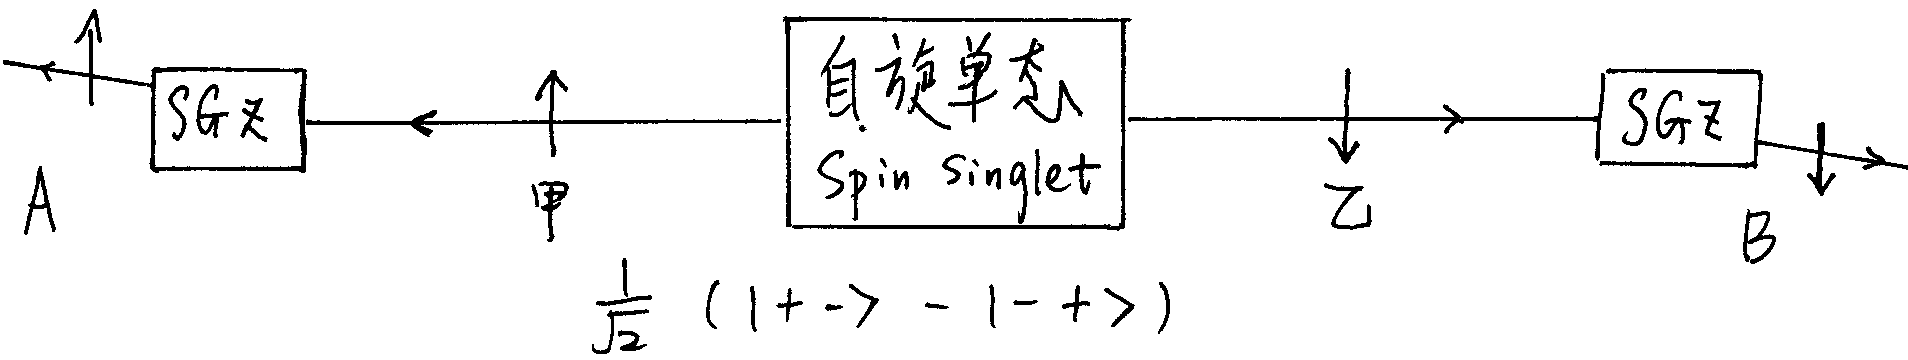
\includegraphics[width=11cm]{DiracNotation/EPRspinsinglet.png}
\caption{自旋相关实验}
\label{default}
\end{center}
\end{figure}

我们在想象中做以下实验:

\begin{enumerate}
\item 

A在左侧不对甲自旋做任何测量,B在右侧对乙自旋测量它在z方向的取值,向上或向下,结果是完全随机的。这里我们没有找到任何物理现实。

\item

A在左侧对甲自旋测量它在z方向的取值,向上或向下,也是随机的;在A完成测量的瞬间,B在右侧对乙自旋也做z方向的测量,在B看来其结果也是随机的,没有任何规律,但如果我们把A和B的测量结果汇总在一起看的话,我们就能发现A和B的测量结果存在着关联,而且是完全的百分百的关联。

比如:只要甲是向上,那么乙就一定是向下;如果甲向下,那乙就一定向上。我们可以把那些使乙确定地“几率为一”地取向上或向下的情形汇总在一起。首先这就符合了爱因斯坦对“物理现实”的定义,这里一定存在一个自旋在z方向上的物理现实。其次量子态比我们设想的要复杂,看起来都叫一个名字,但却可进一步分成很多类,有的自旋向上,有的自旋向下……

\item

我们还可以让A、B都对自旋的x分量进行测量。将得到完全一样的结果。即看起来B对乙自旋x分量的测量是完全随机的,但如果我们把A和B的测量结果拿到一起汇总的话,我们就可以发现对某些测量,B对乙自旋的测量是确定地为向左或向右。Again,按照爱因斯坦对物理现实的定义,自旋的x分量也是“物理现实”的一个要素。

\end{enumerate}

这里要做一个重要的声明,就是我们总是让A先对甲自旋进行测量,而B对乙自旋的测量是在A完成测量的瞬间进行的。如此设计的理由是要保证A在左侧进行的观测——某种扰动——不会影响传播到乙自旋所在的右侧。这样我们可以心安理得的认为B在右侧面对的是同一个量子态。但现在我们所说的量子态必须做集合理解,集合里面有很多假想的乙自旋的态,它们各自又可以分成不同的类,以对应那些可以确定取值的实验。(用物理的术语讲,这个集合就叫系综ensemble)

爱因斯坦这里用到了“定域原则”,即对空间分离的两个系统甲和乙,乙的任何变化不是对甲操作的结果。

如果坚持“定域原则”的话,$S_x$和$S_z$就可以同时是物理现实了,原则上我们可以给系综里的每个自旋指定一个$S_x$的取值,同时一个$S_z$的取值,但我们的量子力学——海森堡、薛定谔和狄拉克的量子力学——无法提供这个信息,在此意义下我们说量子力学是不完备的。

爱因斯坦是这样定义一个物理理论的完备性的:“物理现实的每个要素在物理学理论中都必须有它的对应部分。”

爱因斯坦并不认为量子力学是错的,但他认为量子力学是不完备的,即潜在地还存在着一个升级的版本可以使每个“物理现实”的要素都在理论中有对应,在我们现在的例子下就是$S_x$和$S_z$。

爱因斯坦这里其实是要做一个选择,即在“定域原则”和“不确定原理”之间选择。坚持了“定域原则”,就意味着我们构造了一个$S_x$和$S_z$都要取确定值的例子,这就必须放弃“不确定原理”。

放弃“定域原则”,意味着A在左侧的测量动作会在瞬间对远在右侧的乙自旋进行筛选,即瞬间B所面对的乙自旋的态就发生变化了。我们仍可按海森堡-薛定谔-狄拉克的量子力学对它进行处理,投影到基矢上,并计算几率幅。

放弃“定域原则”并不意味着违反相对论,因为B仅在它的局域进行测量,无法同时知道A对甲自旋的测量结果,所以不论有没有百分百的自旋相关,在B看来它测得的结果都是完全随机的结果,没有任何意义。换句话说我们无法利用纠缠态进行通讯,所以也谈不上违反相对论。

仅仅如此我们是无法判断孰是孰非的。因为爱因斯坦及后来隐变量理论的主张者都没提出替代性的量子理论,所以很难构造实验去进行判定。

\subsubsection{贝尔不等式}

我们同意无法同时确定$S_x$和$S_z$,但假设有很多自旋1/2,我们把$S_z$和$S_x$的取值同时赋予这些自旋,并对它们进行分类,比如我们有(z+,x-),这意味着如果我们对这类自旋测量$S_z$的话,我们将确定地得到向上;我们也可以选择测量$S_x$,确定地得到向下。除了(z+,x-),我们还有相同数量的自旋属于(z+,x+)类。假如我们对筛选出来的$z+$自旋测量$S_x$,50\%的可能性得到$x+$,另外50\%的可能性得到$x-$。

考虑自旋单态(总自旋为0的态),假设自旋可以用(z+,x-)这样的记号进行分类的话,那么(z-,x+)和(z+,x-)就构成一对。总共有四种可能性:

\begin{description}
\item[类型 I:] 

甲(z+,x-);乙(z-,x+)

\item[类型 II:] 

甲(z+,x+);乙(z-,x-)

\item[类型 III:]

甲(z-,x+);乙(z+,x-)

\item[类型 IV:]

甲(z-,x-);乙(z+,x+)

\end{description}

这里对左侧的甲自旋,假如属于第I种类型,A可以对甲测量$S_z$,也可以测量$S_x$,但这些动作都不会改变右侧的乙自旋(z-,x+),这就构造了一个符合爱因斯坦“定域原则”的方案。

进一步讨论,假如A先对甲测量$S_z$,假设结果是向上,这筛选出类型I和类型II,但这个测量动作之后甲和乙就不再是自旋单态了。如果我们再继续对甲测量$S_x$,对乙也测$S_x$,它们的测量结果将失去关联。

在此基础上我们可以讨论贝尔不等式(Bell's inequality)。贝尔不等式是贝尔在1964年提出来的,他构造了一个可以区分正统量子力学和符合“定域原则”替代版本量子力学的实验判据。

其实没有替代版本的量子力学,需要做的是把“定域原则”以某种方式考虑进去。

考虑三个互相不正交的方向:a,b和c。我们可以沿a,b或c的方向测量自旋。然后假设有甲、乙两个自旋,甲向左飞,乙向右飞。

甲和乙构成自旋单态,这意味着如果我们可以用(a-,b+,c+)对甲进行标记的话,那么与甲对应的乙就只能是(a+,b-,c-)。

甲、乙构成的自旋单态可以分为如下八类,每一类的数字用$N_i$表示:

\begin{description}
\item[$N_1$:] 

甲(a+,b+,c+);乙(a-,b-,c-)

\item[$N_2$:]

甲(a+,b+,c-);乙(a-,b-,c+)

\item[$N_3$:]

甲(a+,b-,c+);乙(a-,b+,c-)

\item[$N_4$:]

甲(a+,b-,c-);乙(a-,b+,c+)

\item[$N_5$:]

甲(a-,b+,c+);乙(a+,b-,c-)

\item[$N_6$:]

甲(a-,b+,c-);乙(a+,b-,c+)

\item[$N_7$:]

甲(a-,b-,c+);乙(a+,b+,c-)

\item[$N_8$:]

甲(a-,b-,c-);乙(a+,b+,c+)

\end{description}

这里所有的N都是非负的,我们可以构造如下不等式:

\begin{equation}
N_3 + N_4 \le N_2 + N_4 + N_3 + N_7
\end{equation}

假设我们做这样的实验:A对甲自旋进行测量,让甲通过a方向的非均匀磁场,得到的结果是向上;然后B对乙自旋进行测量,让乙通过b方向的非均匀磁场,假设得到的结果也是向上。如此关联的测量结果对应的数目是:

\begin{equation}
N_3 + N_4
\end{equation}

我们把这个类型记为(a+,b+),得到这个结果的几率是:

\begin{equation}
P(a+, b+) = \frac{N_3 + N_4}{ \sum\limits_i N_i}
\end{equation}

类似地,A对甲自旋进行测量,让甲通过a方向的非均匀磁场,得到的结果是向上;然后B对乙自旋进行测量,让乙通过c方向的非均匀磁场,假设得到的结果也是向上。我们把这个类型记为(a+,c+),对应的几率是:

\begin{equation}
P(a+, c+) = \frac{N_2 + N_4}{ \sum\limits_i N_i}
\end{equation}

还有(c+,b+),对应的几率是:

\begin{equation}
P(c+, b+) = \frac{N_3 + N_4}{ \sum\limits_i N_i}
\end{equation}

这样我们得到一个关于几率的不等式:

\begin{equation}
P(a+, b+) \le P(a+, c+) + P(c+, b+)
\end{equation}

以上是考虑了“定域原则”后的一个不等式。正统量子力学不考虑“定域原则”,但我们可以利用投影直接把以上几率都计算出来。

以a方向为参照,自旋单态可表示为(总自旋为0,同时总自旋在a方向上的分量为0):

\begin{equation}
\left| spin-singlet \right\rangle = \frac{1}{\sqrt{2}}\left( \left|{a+, a- }  \right\rangle  - \left|{a-, a+ }  \right\rangle \right)
\end{equation}

首先我们计算$P(a+, b+)$,a+是对自旋甲而言的,自旋乙就应处于a-的状态,我们需要算的就是一个a-态下的自旋向b+方向投影:

\begin{equation}
\left\langle {b+} | {a-} \right\rangle = \frac{1}{\sqrt{2}} \cos \frac{\pi - \theta_{ab}}{2} 
\end{equation}

这里$\theta_{ab}$指的是方向a和方向b之间的夹角。

\begin{equation}
P(a+, b+) = \left| {\left\langle {b+} | {a-} \right\rangle} \right|^2 = \frac{1}{2} \sin^2 \frac{\theta_{ab}}{2}
\end{equation}

假如正统量子力学也符合贝尔不等式的话,我们应该有:

\begin{equation}
\sin^2 \frac{\theta_{ab}}{2} \le \sin^2 \frac{\theta_{ac}}{2} + \sin^2 \frac{\theta_{cb}}{2}
\end{equation}

我们可以举一个特例来说明贝尔不等式是被违背的,假设a、b和c都在一个平面内,$\theta_{ab} = 2 \theta$,c正好在a和b的中间,$\theta_{ac} = \theta_{cb} = \theta$。考虑$\theta$的取值范围是0到$\frac{\pi}{2}$,我们可以做个表来说明:

%%%%

\begin{table}[htdp]
\caption{量子力学的计算与贝尔不等式不符}
\begin{center}
\begin{tabular}{|c|c|c|}
\hline
$\theta$ &  $\sin^2 \frac{\theta_{ab}}{2}$  & $\sin^2 \frac{\theta_{ac}}{2} + \sin^2 \frac{\theta_{cb}}{2} $ \\
\hline
$\frac{\pi}{20}$ & 0.024  & 0.012  \\
$\frac{\pi}{10}$ & 0.095  & 0.049  \\
$\frac{3\pi}{20}$ & 0.206  & 0.109  \\
$\frac{\pi}{5}$ & 0.345  & 0.191  \\
$\frac{\pi}{4}$ & 0.5  & 0.293  \\
$\frac{3\pi}{10}$ & 0.654  & 0.412  \\
$\frac{7\pi}{20}$ & 0.793  & 0.546  \\
$\frac{2\pi}{5}$ & 0.904  & 0.69  \\
$\frac{9\pi}{20}$ & 0.975  & 0.843  \\
\hline
\end{tabular}
\end{center}
\label{default}
\end{table}%



%%%%

正统量子力学做出了与符合“定域原则”替代理论完全不同的预言。

这样,我们就可以利用实验去验证爱因斯坦的观点了。

迄今为止的实验都表明贝尔不等式被违反了,在这个意义下我们说量子力学是个“非定域”的理论,对一个纠缠态,某个局部的测量会影响空间分离的另一个局部的状况,这是一种超越距离的瞬时的量子态的坍缩。

那么我们可以通过这种超越距离的瞬时的量子态的改变传递信息吗?比如我们把A、B测量结果100\%相关的情形看做是编码1,而把A、B测量结果一点都不相关的情形定义为编码0,这种方案会奏效吗?正像我们前面讨论过的,B在他的局域,总是面对一组完全随机的测量结果,除非同时他能有A的测量结果并汇总为表格,否则他是没法判断A、B的测量结果是否存在关联的。那么A如何把她的测量结果瞬时传递给B呢?除了打电话可能就没有别的办法了\footnote{写这段的时候,正好在微博上看到一个“笑话”,@灰鸽子银水:“量子纠缠态的超距通信时时被人说起。常有的误解是,一对纠缠态的量子,一个状态发生改变,另一个立即改变——这是超越光速的——用我最喜欢的类比来说,这种改变就像是你在中国的妹妹生了个小孩,远在巴黎的你立即在同时成为了舅舅。你称谓的改变同样是超光速的,但需要一个来自你妹妹的电话才会知道。”}。

这就相当于是在加密传输信息,解密需要的密码本必须预先放在B的手上,他才能解读,但很可惜解密用的密码本不是预先生成的,它是伴随着A对甲自旋的测量临时生成的,A没办法把密码本送过去,B就没法解读他的测量结果中所蕴涵的信息。

~

虽然爱因斯坦在这个问题上判断错误,但我们不能因此就小觑(undervalue)了爱因斯坦的贡献,一个伟大物理学家的错误理论往往比一个平庸物理学家的正确理论对学科的贡献大的多得多。(这意味着在物理学中追求新颖比追求正确更有价值。)

阅读爱因斯坦1935年的论文,我们能够感受到爱因斯坦强健的物理思维,即把哲学的立场——对“物理现实”的坚持——翻译为物理的选择——保留“定域原则”,还是保留“不确定原理”——进而挑战量子理论已经完备的正统观点。

爱因斯坦的这个工作也被看做是今天热门的量子信息学的奠基工作,这篇论文在物理评论网站上显示已经被引用了4249次,而获得了诺贝尔奖的康普顿散射的论文也才仅仅被引用了210次。




\subsection*{练习}

\begin{enumerate}
\item 

氢原子的波函数可以表示为:

\begin{equation*}
\Psi = \frac{1}{\sqrt{14}} \left[ 2 \psi_{100} - 3 \psi_{200} + \psi_322  \right],
\end{equation*}

电子处在态$(100)$,$(200)$,$(322)$的几率分别是多少?假如我们对态$\Psi$测量能量$E$,角动量的平方$L^2$,和角动量的第三分量$L_z$,它们的期望值各是多少?

\item

考虑两个自旋1/2组成的系统,处在态

\begin{equation*}
\left| \alpha \right\rangle = a \left| ++ \right\rangle + b \left| +- \right\rangle + c \left| -+ \right\rangle  + d \left| -- \right\rangle
\end{equation*}

这里态$\left| \alpha \right\rangle $是归一的,即$|a|^2 + |b|^2 + |c|^2 + |d|^2 = 1$。针对这个态测量物理量$S^2$,这里$S$表示总自旋算符,$S = S_1 + S_2$。求:

\begin{enumerate}
\item 

力学量$S^2$的可能测量值是多少?

\item

对每个测量值,它们的概率是多少?(用$a, b, c, d$表示)

\end{enumerate}

\item

$n$是沿空间某方向上的单位向量,它与$z$轴的夹角是$\theta$,它在$x-y$平面上的投影与$x$轴的夹角是$\phi$。

对自旋1/2,求$S \cdot n$的本征值问题。

\begin{figure}[htbp]
\begin{center}
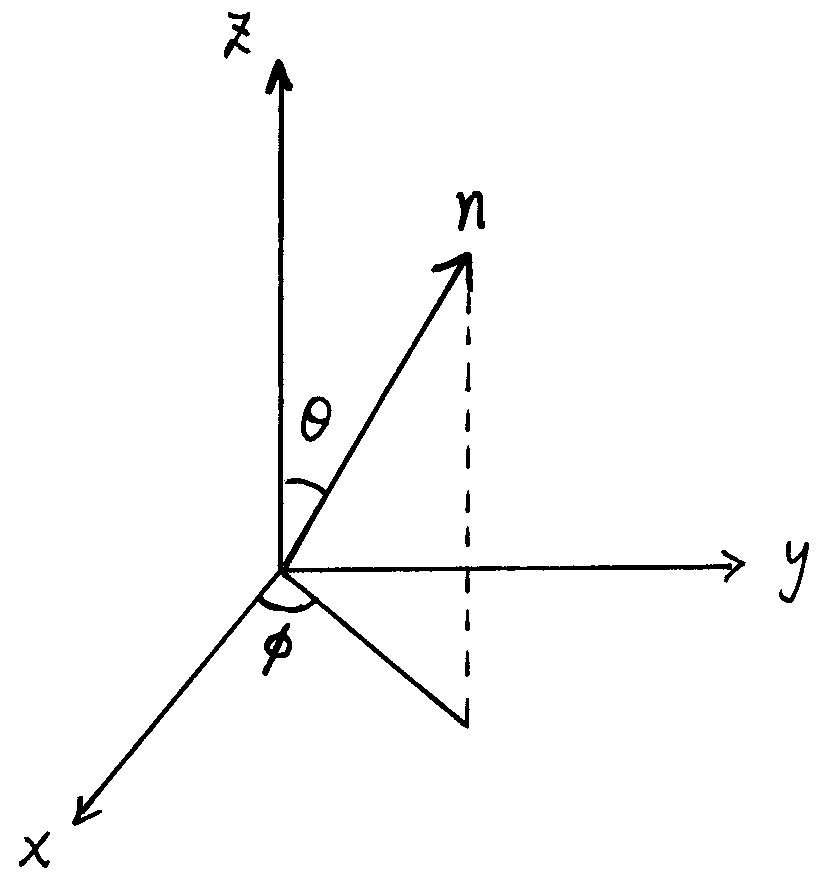
\includegraphics[width=6cm]{DiracNotation/sigma_n.png}
\caption{$n$与$z$轴的夹角是$\theta$,$n$在$x-y$平面上的投影与$x$轴的夹角是$\phi$。}
%\label{default}
\end{center}
\end{figure}


\end{enumerate}